Este anexo reúne las figuras citadas en el cuerpo del informe, en el orden en que aparecen.

\begin{figure}[H]
\centering
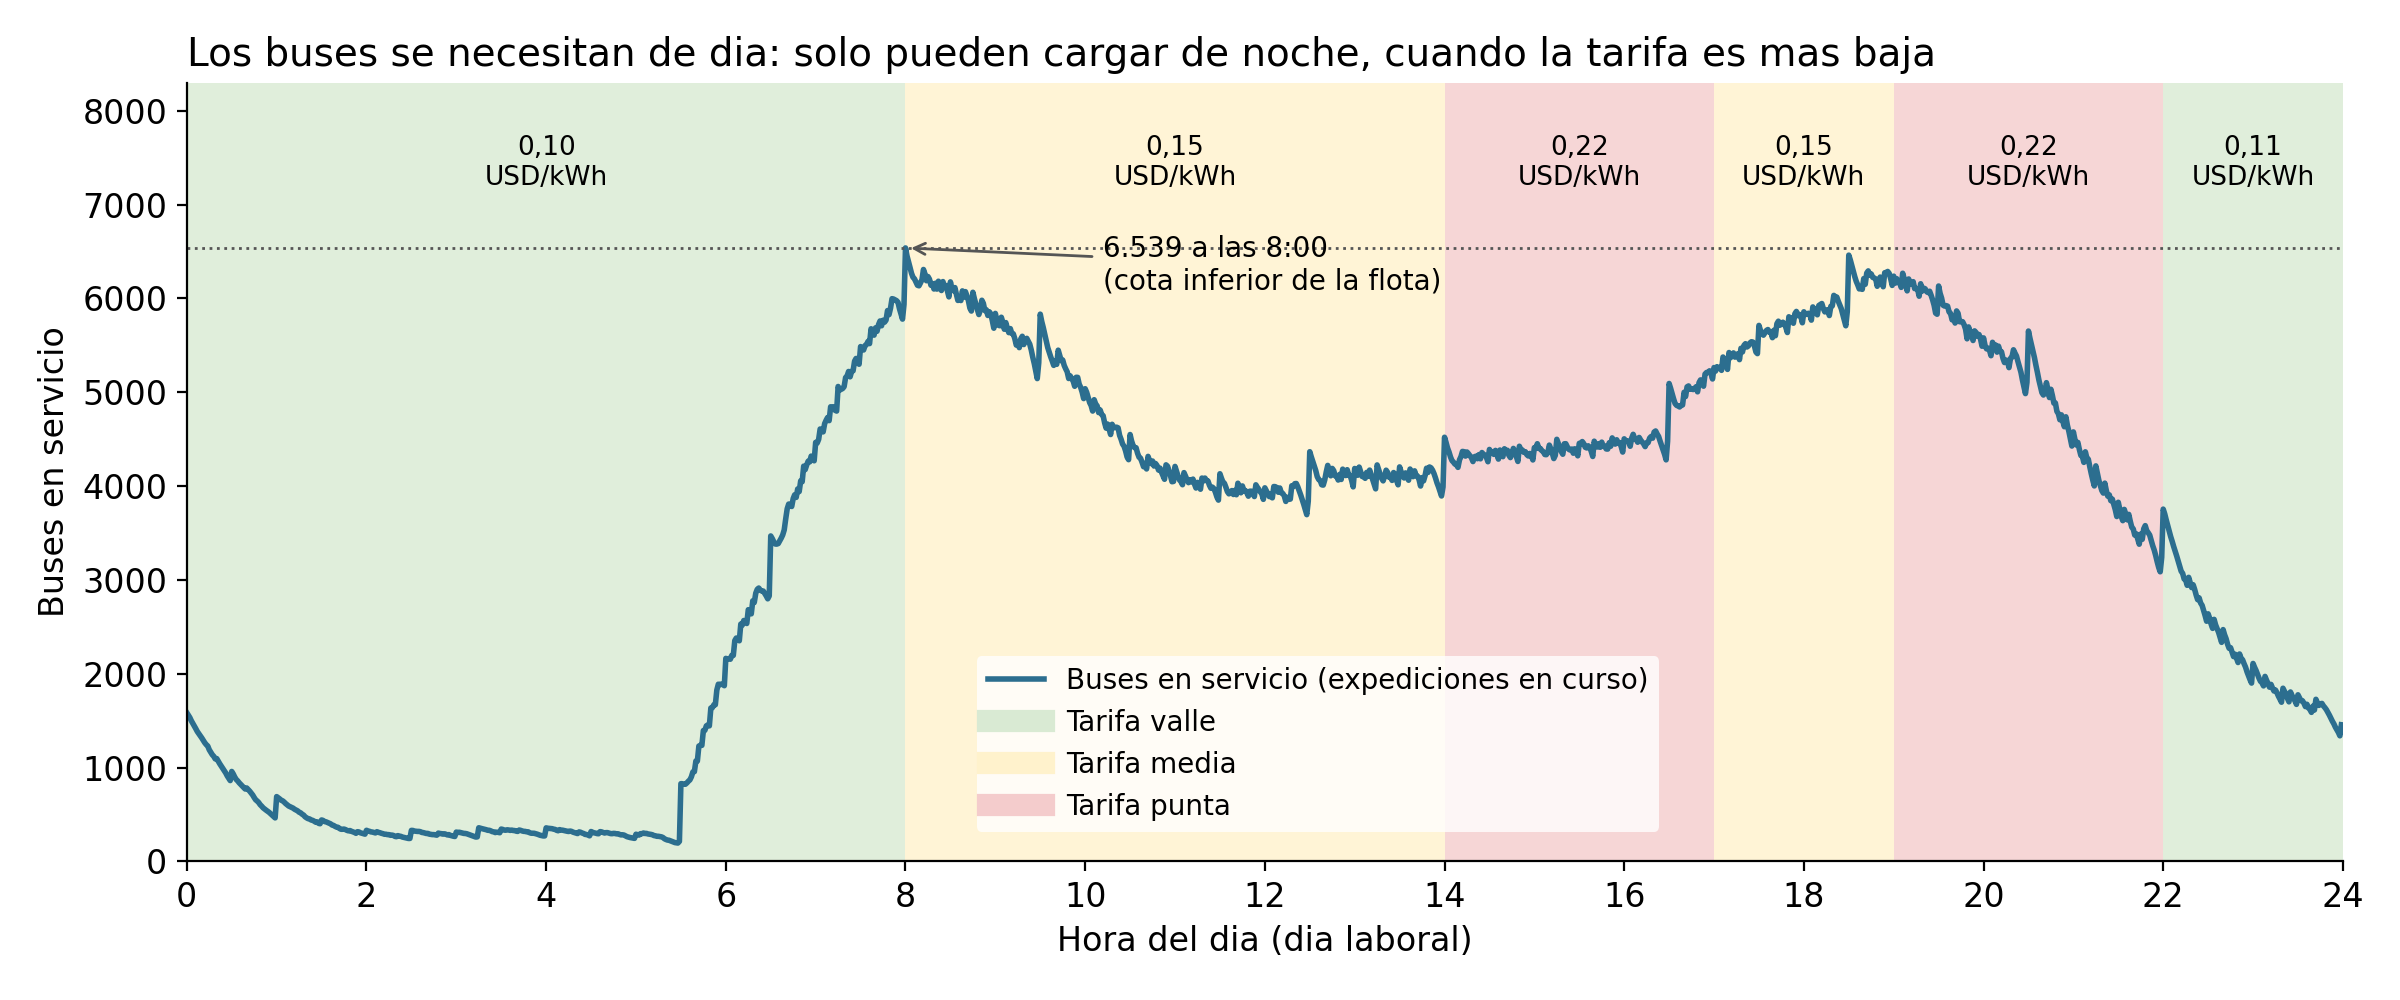
\includegraphics[width=\textwidth,height=0.8\textheight,keepaspectratio]{figures/G1_demanda_y_tarifa.png}
\caption{Expediciones en curso durante el día laboral y tarifa eléctrica por tramo horario.}
\label{fig:demanda-tarifa}
\end{figure}

\begin{figure}[H]
\centering
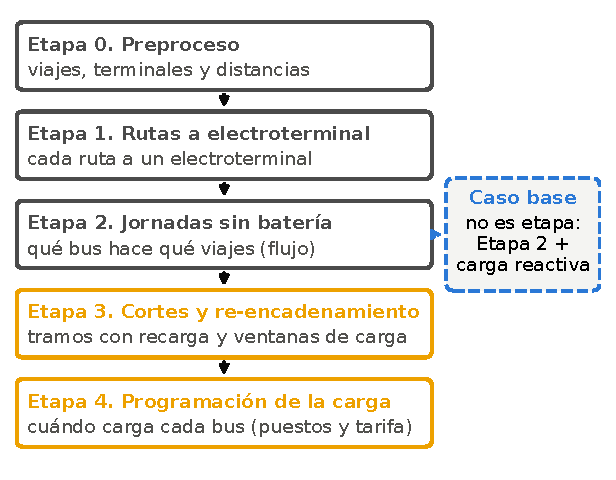
\includegraphics[width=0.7\textwidth,height=0.7\textheight,keepaspectratio]{figures/F1_metodologia.pdf}
\caption{Metodología en cuatro etapas.}
\label{fig:metodologia}
\end{figure}

\begin{figure}[H]
\centering
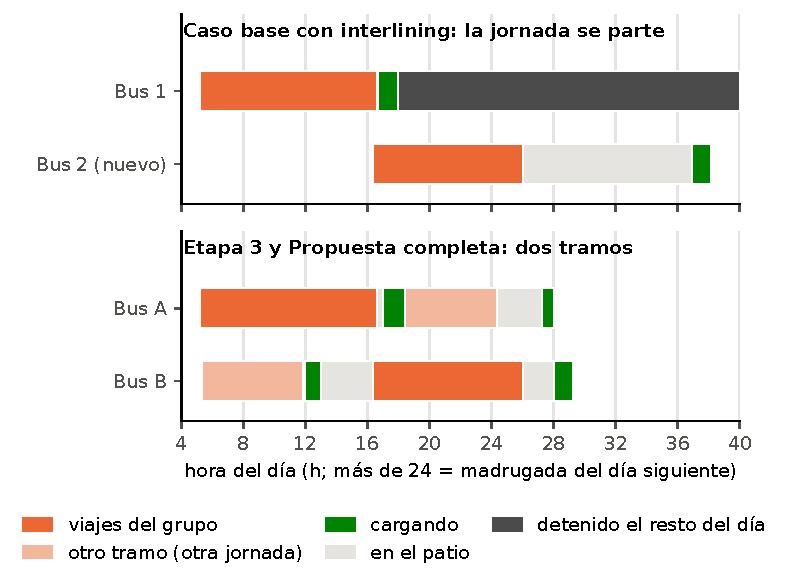
\includegraphics[width=0.8\textwidth,height=0.8\textheight,keepaspectratio]{figures/F2_gantt_jornada.pdf}
\caption{Una jornada de La Reina con la carga reactiva del caso base con \textit{interlining} y con la Etapa 3.}
\label{fig:gantt}
\end{figure}

\begin{figure}[H]
\centering
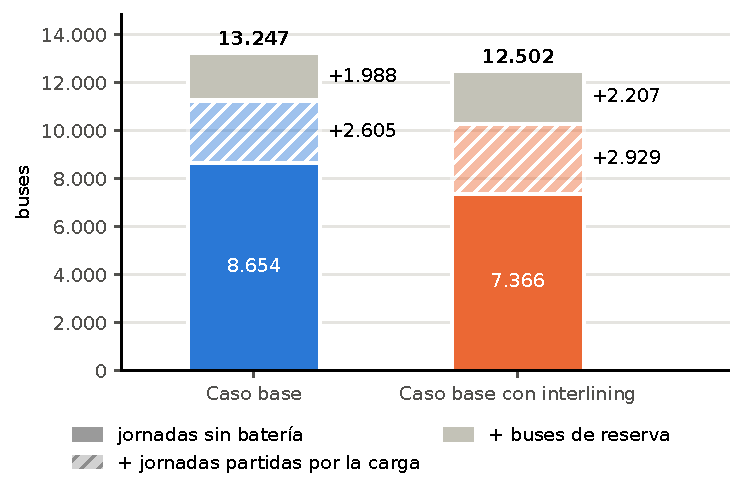
\includegraphics[width=0.8\textwidth,height=0.8\textheight,keepaspectratio]{figures/F0_caso_base_red.pdf}
\caption{Flota del caso base y del caso base con \textit{interlining} en toda la red, sin batería y con carga reactiva.}
\label{fig:caso-base-red}
\end{figure}

\begin{figure}[H]
\centering
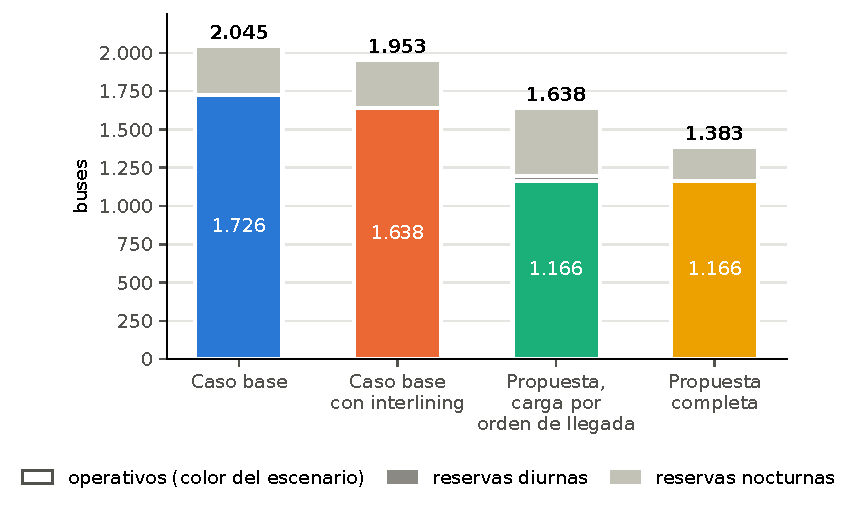
\includegraphics[width=0.8\textwidth,height=0.8\textheight,keepaspectratio]{figures/F3_escalera_buses.pdf}
\caption{Número de buses de los cuatro escenarios en La Reina.}
\label{fig:escalera}
\end{figure}

\begin{figure}[H]
\centering
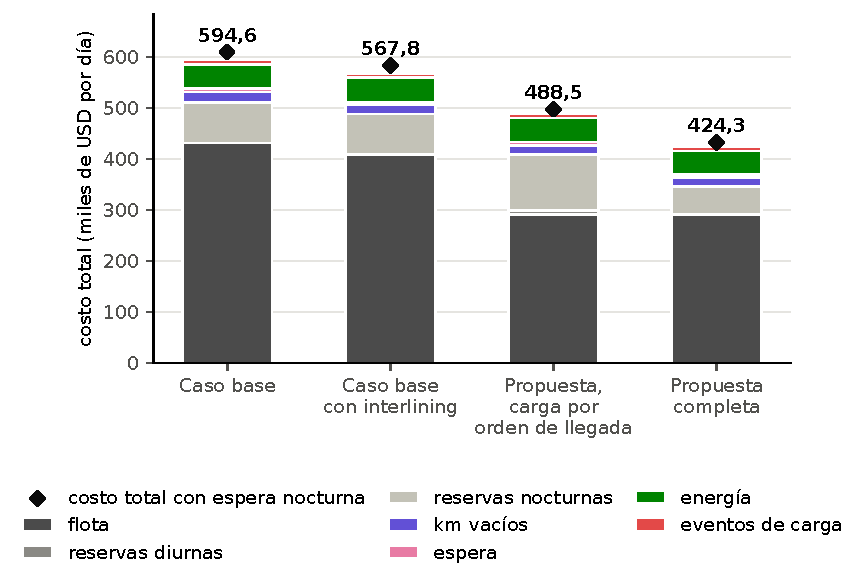
\includegraphics[width=0.8\textwidth,height=0.8\textheight,keepaspectratio]{figures/F4_costo_total.pdf}
\caption{Costo total de los cuatro escenarios en La Reina.}
\label{fig:costo}
\end{figure}

\begin{figure}[H]
\centering
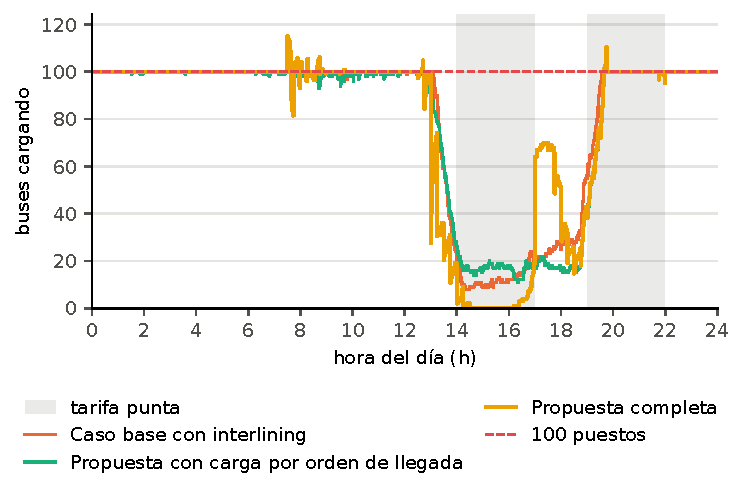
\includegraphics[width=0.8\textwidth,height=0.8\textheight,keepaspectratio]{figures/F5_ocupacion_24h.pdf}
\caption{Buses cargando durante el día en La Reina.}
\label{fig:ocupacion}
\end{figure}

\begin{figure}[H]
\centering
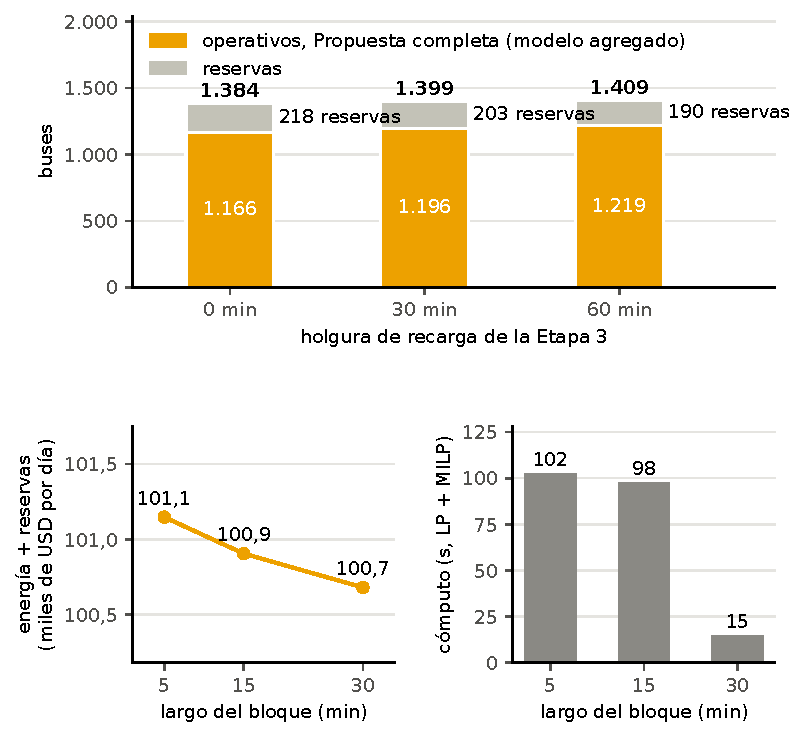
\includegraphics[width=0.8\textwidth,height=0.8\textheight,keepaspectratio]{figures/F6_sensibilidades.pdf}
\caption{Sensibilidad a la holgura de recarga y al largo del bloque (modelo agregado).}
\label{fig:sensibilidad}
\end{figure}
